\documentclass[ShortAfour,times,sageapa]{sagej}
\usepackage[utf8]{inputenc}
\usepackage[T1]{fontenc}
\usepackage{amsmath}
\usepackage{amssymb}
\usepackage{graphicx}
\usepackage{longtable}


\begin{document}
	
\runninghead{Luchman}
\title{Relative importance analysis for count regression models}
\author{Joseph N. Luchman\affilnum{1}}
\affiliation{\affilnum{1}Fors Marsh}

\begin{abstract}
	Count variables are common in organizational science as an outcome. Count regression models (CRMs), such as Poisson regression, are recommended as methods to analyze count variables but can be challenging to interpret given their non-linear functional form. I recommend relative importance analysis as a method to use in intepreting CRM results. This work extends on past research by describing an approach to determining the importance of independent variables in CRMs using dominance analysis (DA). In this manuscript, I review DA as a relative importance method, recommend an $R^2$ to use with CRM-based DA, and outline the results of an analysis with simlulated data that uses the recommended methodology. I also discuss the effect of differential exposure to the count generating process across observations on count outcomes, how to correct for differential exposure, and the effect of differential exposure on relative importance determination. This work contributes to the literature by extending DA to CRMs, discussing the impact of differential exposure on CRM models and relative importance, and for providing a thoroughly documented data analysis that can be used by researchers interested in implementing the methodology.
\end{abstract}

\keywords{Dominance Analysis, Relative Importance, Poisson Regression, Exposure, R-square, Negative Binomial Regression, Count Data, Offset}

\maketitle

\section{Introduction}

	Organizational science often uses how many times a behavior is observed as an outcome to answer research questions. 
	Such behavior counts arise from many different sources at the organization- and individual-level of aggregation.
	Organization-level behavior counts used in the literature include the number of organizations adopting a specific practice in a week \cite{naumovska2021strength} and number of divestitures organizations make in a year \cite{bettinazzi2021stakeholder}. 
	Individual-level behavior counts used in the literature include the number of scientific articles published in a year by an academic \cite{rotolo2013does} or number of errors that resulted in an accident in the last three months among medical doctors \cite{naveh2015active}.
	Behavior counts such as the above examples are valuable outcomes given that organizational science concepts are often defined terms of behavior \cite(e.g., job performance;){motowidlo2003job} and strategies to validate outcomes often use observable behavior as an outcome \cite(e.g., criterion-oriented validity;){cronbach1955construct}.
	
	The conceptual value of behavior counts as outcomes aside, data analysis with behavior counts as a dependent variable/DV require the use of specialized tools.
	The recommended data analysis strategy with behavior counts uses regression models designed for non-negative integer or count distributions \cite(e.g.,){blevins2015count}.
	These count regression models/CRMs include the Poisson regression/PR and negative Binomial regression/NBR models.
	Both PR and NBR are commonly used in the organizational science literature and implemented in many data analytic software environments.
	
	CRMs are generalized linear models that mathematically transform the predictive equation to ensure that predicted values stay in the range of the DV.
	CRMs use an exponential or log-linear transformation that has the form $y = e^{\beta}$. 
	Thus the predictive equation represented by $\beta$ requires back-transformation using a natural logarithm in order to obtain a predicted count value.
	This log-linear transformation ensures that predicted values from $\beta$ can take on any number in the real number line yet, when back-transformed into predicted counts, will have a lower bound of 0.
	
	The log-linear predictive equations and coefficients CRMs estimate are challenging to interpret directly.
	Log-linear CRM coefficients are challenging to interpret because they describe how the natural logarithm of the DV changes given a 1 unit change to an independent variable/IV. 
	When back-translated through an exponential function, CRM coefficients are known as incidence rate ratios and describe the percentage change in the DV per unit change to the IV.
	Importantly, the percentage change described by CRM coefficients makes the count values produced by those changes relative to where they began.
	For example, a CRM coefficient does not differentiate between a change from 1 predicted behavior to 2 and 5 predicted behaviors to 10. 
	Despite the noteworthy difference in the absolute number of behaviors in both examples, each describe a 100\% increase in the count DV value.
		
	Model post-estimation methods such as graphing estimated marginal means are useful interpretive tools for log-linear CRMs to better contextualize the logarithmic predicted values they produce.
	Another increasingly common model post-estimation tool used to contextualize model predictions are relative importance analysis methods \cite{tonidandel2011relative}. 
	Relative importance analysis methods focus on how different IVs in the model contribute to the $R^2$ as computed by methods such as dominance analysis/DA \cite{azen2003dominance}.
	
	To date, published methodological work has extended DA from the linear regression model/LRM on which it was originally developed, to generalized linear models including binary \cite{azen2009using}, ordered, and multinomial logit models \cite{luchman2014relative}.	
	This work extends DA to CRMs and makes three contributions to the literature.
	This work first reviews DA as a relative importance methodology, recommends using a specific pseudo-$R^2$ statistic for CRM-based DA, and implements multiple data analytic examples of DA with that statistic.
	The pseudo-$R^2$ chosen for CRM-based DA is a direct generalization of the explained variance $R^2$ in the LRM to generalized linear models based on model deviance.
	The data analytic examples then use this deviance-based pseudo-$R^2$ as the fit statistic in a series of DA computations with simulated Poisson and negative Binomial distributed data.
	
	Second, this work discusses data generation mechanisms with count DVs and outlines how research questions with count DVs can, under certain circumstances, be affected by a concept known as differential exposure.
	Differential exposure is a concept whereby two observations have different numbers of opportunities to produce behavior counts.
	Oftentimes such differential exposure is a nuisance factor related to data collection context, not of substantive interest, and is correctable in the model using an offset term with a variable measuring differential exposure.
	As I will show in this work, differential exposure is of particular import for DA statistic computation as it can affect estimates of DA statistics even when model coefficients are relatively unaffected.
	
	Finally, this work extends on that of Blevins, Tsang, and Spain \citeyear{blevins2015count}'s review and recommendations for the use of CRMs in organizational science. 
	Blevins et al. discuss the extent of CRM use in the organizational science literature, describe model and analytic details about the PR and NBR models, and provide a flowchart that researchers can use to identify which CRM might be best to choose for their data analysis.
	In this work, I extend on their review to add an in-depth discussion of DA and its role as a post-estimation methodology.
	DA extends on the interpretation of coefficients to describe how the coefficients, when applied to the observed data, improve model-to-fit in predicting the count DV.
	In addition, the discussion of differential exposure extends on Blevins et al.'s conceptual review to cover an additional consideration important for CRM-based data analysis.
	
	I begin the manuscript with a detailed discussion of the conceptual background of DA--the relative importance analysis method most applicable to CRMs.	
 	Here I discuss the different levels of dominance between two IVs as defined by DA, how these levels are determined in the data, and what this level of dominance means in terms of the importance of any IV in the model.
	The conceptual discussion of DA is followed by a more focused discussion where I apply DA to CRMs.
	The goal of the focused CRM-based DA discussion is to recommend a model fit statistic for use in dominance designations.
	In the third section, I apply the topics discussed in the previous two sections in a detailed PR-based DA using simulated data designed be useful in illustrating key CRM-based DA concepts.
	In a fourth and final section, I turn to discussing the concept of differential exposure in count DVs, show how it can affect results from CRM analysis, and provide the method used to correct for it in analysis.
	My goal in discussing differential exposure is to outline the effect of this concept on DA statistics and designations.
	To this end, I compute and compare CRM-based DA statistics with and without corrections to illustrate the impact of ignoring this issue during analysis.
	
	% ended here
		
\section{Dominance Analysis: A Unique Relative Importance Analysis Method}

	Research methodologists and statisticians have used many methods over the years to determine how important an IV is in a LRM \cite(see reviews in){gromping2007estimators, johnson2004history}.
	Importance methods have included the correlation between the IV and DV, an IV's standardized regression coefficient, as well as the increment to the $R^2$ makes, an IV makes when predicting the DV.
	These methods, however informative in specific circumstances, are not considered to be useful as importance metirics as they fail to simultaneously account for the IV's bivariate and multivariate (i.e., controlling for other IV) relationships with the DV \cite{johnson2004history}.
	Accommodating both bi- and multivariate relationships is important in determining importance as, for most statistical models, the order in which IVs are included is arbitrary yet the order of inclusion of IVs fundamentally affects the inferences made about IV importance.
	Hence, it is essential to use importance methods that are independent of inclusion order.
	
	One importance method that is independent of ordering and has been favorably received in the methodology community, is DA.
	DA was originally developed as a method for determining IV importance for the LRM by Budescu \citeyear{budescu1993dominance} that extended on past methods by defining importance in terms of pairwise IV comparisons as inferred from the direct comparison of sub-model $R^2$ values.
	Sub-model $R^2$ are those computed by re-fitting the model to the data with some subset of all the IVs.
	In a model with $p$ IVs there are a total of $2^p$ sub-models including the full model with all $p$ IVs and the null model with none of the IVs (i.e., an intercept-only model)--which always produces a value of 0 and is often omitted.
	DA achieves order independence by comparing the two focal IVs' $R^2$ values across sub-models that contain all combinations of the non-focal IVs including the null set of no other non-focal IVs.	
	In this way, the dominance comparisons produced by DA do not depend on the order of IV inclusion and, indeed, require that an IV obtain a higher value than another IV irrespective of inclusion of other non-focal IVs.
	
	As an example of how the dominance comparison is implemented, consider a model with 4 IVs: $IV_x$, $IV_z$, $IV_w$ and $IV_v$ predicting $Y$.
	If the dominance comparison was focusing on $IV_x$ versus $IV_z$, there would be a total of 3 possible $R^2$ comparisons each of which is outlined below in Table \ref{tab:exdom}.
	In each comparison, the subscripted model indicates the form of the LRM equation in symbolic form (i.e., similar to an R formula interface).
	$IV_x$ dominates $IV_z$ only when all the sub-model $R^2$ values that include $IV_x$ are greater than the sub-model $R^2$ values that include $IV_z$ across all three of these sub-models.
	The dominance comparison described in this section has, more recently, been named complete dominance and has been recognized as the most stringent, or hardest to achieve, dominance designation in a series of three possible designations \cite{azen2003dominance}.	

		\begin{table}[h!]
			\centering
			\caption{\centering Example Dominance Comparisons}
			\begin{tabular}{ l | l l }
				
				& Sub-model with $IV_x$ & Sub-model with $IV_z$ \\
				\hline
				Across null set/no other IVs & $R^2_{Y \sim IV_x}$ & $R^2_{Y \sim IV_z}$ \\
				Comparing across $IV_w$ & $R^2_{Y \sim IV_x + IV_w}$ & $R^2_{Y \sim IV_z + IV_w}$ \\
				Comparing across $IV_v$ & $R^2_{Y \sim IV_x + IV_v}$ & $R^2_{Y \sim IV_z + IV_v}$ \\
				Comparing across both $IV_w$ and $IV_v$ & $R^2_{Y \sim IV_x + IV_w + IV_v}$ & $R^2_{Y \sim IV_z + IV_w + IV_v}$ \\
				\hline
		\end{tabular}
		\label{tab:exdom}
	\end{table}
	
	\subsection{Complete Dominance}
	
	Complete dominance is the most stringent of the dominance designations as it is a difficult designation for an IV to achieve over another.
	Complete dominance is difficult to achieve as it involves direct comparisons between IVs at the level of individual sub-models' $R^2$ values.
	The reason this designation is so difficult to achieve is that it is non-compensatory; all sub-model $R^2$ value comparisons must favor one IV over another or the designation will fail to be achieved.
	
	The process for determining complete dominance between two IVs, $IV_x$ and $IV_z$ with an arbitrary number of IVs in the model ($p$) can also be defined as:
	
	\begin{equation}
		IV_x \, D \, IV_z \quad if \quad k = \sum^k_{j=1} \Biggr\{ \begin{matrix} if \ R^2_{Y \sim IV_x + \{u_j\}} > R^2_{Y \sim IV_z + \{u_j\}} \ then \ 1 \\ else \ 0 \end{matrix}
		\label{eq:cptdom}
	\end{equation}
	
	Where the total number of combinations of IVs not including $IV_x$ or $IV_z$ is $k = 2^{p - 2}$ and $u_j$ is a distinct subset of the other $p - 2$ IVs.
	The braces surrounding $u_j$ indicate that it is a subset of IVs such as those in Table \ref{tab:exdom}.
	The $D$ in this case is a designation indicating complete dominance of the left hand IV over the right hand IV.
	
	Ultimately, if $IV_x$ completely dominates $IV_z$ as is outlined in Equation \ref{eq:cptdom}, $IV_x$ has bested $IV_z$ 
	in all possible directly comparable ways in the model.
	As such, when $IV_x$ completely dominates $IV_z$, it clearly explains more of $Y$, and is thus more important for explaining differences observed in $Y$, in the model
	
	Because complete dominance is a difficult criterion to achieve in comparing two IVs, alternative, less-stringent and more compensatory, dominance designations have been proposed to provide more ways to compare the predictive usefulness of IVs against one another.
	The criteria used in the sections to come involve averaging the $R^2$ values associated with the IVs in the comparison and comparing those resultant averages.
	
	\subsection{Conditional Dominance}
	
	A less stringent dominance designation between IV pairs than complete dominance is called conditional dominance.
	Conditional dominance relaxes the stringency of the comparisons across pairs of IVs by changing the focus from comparing $R^2$ values of individual sub-models to averages of $R^2$ increments across sub-models.
	By comparing averages of $R^2$ increments, as opposed to individual sub-model $R^2$ values, conditional dominance allows for some sub-models with higher values of $R^2$ increments to compensate for sub-models with lower values of $R^2$ increments in the averaging.
	Thus, it is more likely that an IV will be determined to be conditionally dominant over another given a set of sub-model $R^2$ values.
	
	The specific comparisons made to determine conditional dominance of one IV over another focus on the average increment an IV makes to the $R^2$ with a specific number of IVs in the sub-model.
	The averages are aggregated by the number of IVs in the sub-model as it is necessarily the case that, as more IVs are added to a model, the incremental contribution any one IV can make to the $R^2$ shrinks.
	Hence, conditional dominance designations acknowledge that increments to the $R^2$ are best compared in the context of the number of IVs in the model.	
	
	The average increments to the $R^2$ computed for determining conditional dominance are known as conditional dominance statistics.
	Each IV has a conditional dominance statistic for each number of IVs in the sub-model. 
	Thus, with $p$ IVs, each IV will have $p$ conditional dominance statistics to compare to another IV.
	Extending on Table \ref{tab:exdom}, determining conditional dominance between $IV_x$ and $IV_z$ would involve all four different conditional dominance statistics the computation of which are outlined below in Table \ref{tab:excdl}.
	
	\begin{table}[h!]
		\centering
		\caption{\centering Example Conditional Dominance}
		\begin{tabular}{ l | l l }
			Comparing at & Average with $IV_x$ & Average with $IV_z$ \\
			\hline
			One IV & $\Delta R^2_{Y \sim IV_x + \{\emptyset\}}$ & $\Delta R^2_{Y \sim IV_z + \{\emptyset\}}$ \\
			\hline
			& $(\Delta R^2_{Y \sim IV_x + \{IV_w\}} + $ & $(\Delta R^2_{Y \sim IV_z + \{IV_w\}} + $ \\
			Two IVs & $\Delta R^2_{Y \sim IV_x + \{IV_v\}} + $ & $\Delta R^2_{Y \sim IV_z + \{IV_v\}} + $ \\
			& $\Delta R^2_{Y \sim IV_x + \{IV_z\}})\frac{1}{3}$ & $\Delta R^2_{Y \sim IV_z + \{IV_x\}})\frac{1}{3} $ \\
			\hline
			& $(\Delta R^2_{Y \sim IV_x + \{IV_w + IV_v\}} + $ & $(\Delta R^2_{Y \sim IV_z + \{IV_w + IV_v\}} + $ \\
			Three IVs & $\Delta R^2_{Y \sim IV_x + \{IV_w + IV_z\}} + $ & $\Delta R^2_{Y \sim IV_z + \{IV_w + IV_x\}} + $ \\
			& $\Delta R^2_{Y \sim IV_x - \{IV_v + IV_z\}})\frac{1}{3}$ & $\Delta R^2_{Y \sim IV_v + \{IV_w + IV_x\}})\frac{1}{3}$ \\
			\hline
			Four IVs & $\Delta R^2_{Y \sim IV_x + \{IV_w + IV_v + IV_z\}}$ & $\Delta R^2_{Y \sim IV_v + \{IV_w + IV_w + IV_x\}}$ \\
			\hline
		\end{tabular}
		\label{tab:excdl}
	\end{table}
	
	The $\Delta$ indicates that the values in Table \ref{tab:excdl} reflect that the $R^2$ value is an increment made by the first IV beyond the subset of IVs in braces.
	For the first set of conditional dominance statistics, at one IV, the $\emptyset$ indicates the null set with no IVs--thus, is the $R^2$ with the IV by itself in a subset.
	Note that the conditional dominance statistics are not only averaged but also include all IVs in their computation.
	Hence, conditional dominance comparisons between two IVs' conditional dominance statistics will include increments from the IV against which they are being compared in their each average.
	This is a noteworthy difference from complete dominance designations that ignore sub-model $R^2$ values that include the IV against which the focal IV is being compared.
	
	The process of computing conditional dominance statistics for $IV_x$ for a number of IVs in the model $i$ can be formalized as in Equation \ref{eq:cdlst} below.
	
	\begin{equation}
		C^{i}_{IV_x} = \frac{\sum^{l_i}_{g=1} \Delta R^2_{IV_x + \{o_g\}}}{l_g}
		\label{eq:cdlst}
	\end{equation}
	
	Where $l_i$ is the number of combinations of size $i$ given $p$ IVs and $o_g$ is a distict subset of the $p$ IVs of size $i - 1$, not inluding $IV_x$, that are included in the sub-model.
	
	The process for determining conditional dominance between two IVs, $IV_x$ and $IV_z$, can also be defined as in Equation \ref{eq:cdldom}.
	
	\begin{equation}
		IV_x \ D_c \ IV_z \quad if \quad p = \sum^p_{i=1} \Biggl\{ \begin{matrix} if \ C^{i}_{IV_x} > C^{i}_{IV_z} \ then \ 1 \\ else \ 0 \end{matrix}
		\label{eq:cdldom}
	\end{equation}
	
	The $D_c$ in this case is a designation indicating conditional dominance of the left hand IV over the right hand IV.
	
	When complete dominance is not achieved between two $IV_x$ and $IV_z$, but conditional dominance is, $IV_x$ tends to explain more of $Y$ than does $IV_z$ irrespective of inclusion order.
	Thus, when achieved, conditional dominance suggests that $IV_x$'s effects are not generally sensitive to the order in which it enters the model compared to $IV_z$ and that it is more important conditional on the number of IVs in the sub-model.
	
	Conditional dominance between two IVs is much less stringent than complete dominance but can still be a difficult designation to meet for IV pairs in models with a great deal of between-IV overlap.
	The final dominance designation involves yet another averaging step to allow reduce the stringency of the comparison and allow for compensation of values over inclusion orders.
	
	\subsection{General Dominance}
	
	The least stringent dominance designation between IV pairs is called general dominance.
	General dominance further relaxes the stringency of the comparisons between IV pairs by changing the focus from comparing average increments grouped by the number of IVs in a sub-model to the arithmetic average of these averages.
	By averaging over conditional dominance statistics, general dominance allows higher contributions at specific numbers of IVs in the sub-model to compensate for lower contributions at other numbers of IVs in the sub-model. 
	The values generated by general dominance almost guarantee that IVs will produce a dominance designation and permits an explicit rank ordering of IV predictive usefulness of each IV in the model.
	
	The averaged conditional dominance statistics computed for determining general dominance are known as general dominance statistics. The single general dominance statistic computed for each IV
	Extending on Table \ref{tab:excdl}, determining general dominance between $IV_x$ and $IV_z$ would involve both general dominance statistics.
	Both general dominance statistics are included below in Table \ref{tab:exgen} in their full computational form.
	
		\begin{table}[h!]
		\centering
		\caption{\centering Example General Dominance}
		\begin{tabular}{ l l }
			Average with $IV_x$ & Average with $IV_z$ \\
			\hline
			$\Delta R^2_{Y \sim IV_x + \{\emptyset\}}\frac{1}{4} + $ & $\Delta R^2_{Y \sim IV_z + \{\emptyset\}}\frac{1}{4} +$ \\
			$(\Delta R^2_{Y \sim IV_x + \{IV_w\}} + $ & $(\Delta R^2_{Y \sim IV_z + \{IV_w\}} + $ \\
			$\Delta R^2_{Y \sim IV_x + \{IV_v\}} + $ & $\Delta R^2_{Y \sim IV_z + \{IV_v\}} + $ \\
			$\Delta R^2_{Y \sim IV_x + \{IV_z\}})\frac{1}{12} + $ & $\Delta R^2_{Y \sim IV_z + \{IV_x\}})\frac{1}{12} + $ \\
			$(\Delta R^2_{Y \sim IV_x + \{IV_w + IV_v\}} + $ & $(\Delta R^2_{Y \sim IV_z + \{IV_w + IV_v\}} + $ \\
			$\Delta R^2_{Y \sim IV_x + \{IV_w + IV_z\}} + $ & $\Delta R^2_{Y \sim IV_z + \{IV_w + IV_x\}} + $ \\
			$\Delta R^2_{Y \sim IV_x - \{IV_v + IV_z\}})\frac{1}{12} + $ & $\Delta R^2_{Y \sim IV_v + \{IV_w + IV_x\}})\frac{1}{12} +$ \\
			$\Delta R^2_{Y \sim IV_x + \{IV_w + IV_v + IV_z\}}\frac{1}{4}$ & $\Delta R^2_{Y \sim IV_v + \{IV_w + IV_w + IV_x\}}\frac{1}{4}$ \\
			\hline
		\end{tabular}
		\label{tab:exgen}
	\end{table}

	As is implied by the computations in Table \ref{tab:exgen}, each general dominance statistics are a weighted average of the individual increments to the $R^2$s.
	
	The process of computing the general dominance statistic for $IV_x$ is formalized below in Equation \ref{eq:genst}.
	
	\begin{equation}
		C_{IV_x} = \frac{\sum^{p}_{i=1} C^i_{IV_x}}{p}
		\label{eq:genst}
	\end{equation}
	
	Using the general dominance statistics computed in Equation \ref{eq:genst}, the process of determining general dominance of $IV_x$ over $IV_z$ can also be defined as in Equation \ref{eq:gendom}.
	
	\begin{equation}
		IV_x \ D_g \ IV_z \quad if \quad C_{IV_x} > C_{IV_z}
		\label{eq:gendom}
	\end{equation}
	
	The $D_c$ in this case is a designation indicating conditional dominance of the left hand IV over the right hand IV.
	
	When complete and conditional dominance is not achieved between two $IV_x$ and $IV_z$, but general dominance is, $IV_x$ tends to explain more of $Y$ than does $IV_z$ but is sensitive to inclusion order.
	Hence, when achieved, general dominance suggests that $IV_x$'s predictive usefulness is on average, better than $IV_z$ and that it is more important when ignoring the effect of inclusion order.
	
	It is important to note that the  general dominance statistic values, when summed across the $p$ IVs, equals the sub-model $R^2$ when all $p$ predictors are included.
	This is a useful feature of these statistics that, as has been discussed in other reviews \cite{gromping2007estimators,johnson2004history}, ties this method to earlier work that has focused on the decomposition of the $R^2$ statistic.

	In the sections above, I have provided a discussion of DA's development and reviewed how DA statistics are computed and DA designations are determined.
	In the section below, I transition from a broad outline of DA to a more targeted discussion of the application of DA to CRMs.
	The focus of the section discussion of CRM-based DA focuses on considering which fit metric should be used when applying DA to CRMs.
	
\section{Applying Dominance Analysis to Count Regression Models}

	A complication of applying DA to CRMs is that most of the literature on DA has focused on its application to LRM with the variance explained $R^2$.
	Given the semi-continuous nature of count DVs and that the output from CRMs is typically in the form of a predicted count/mean value, the $R^2$ could be applied to CRM-based DA.
	
	Although the variance explained $R^2$ could be applied, there are good conceptual reasons to choose another fit metric. 
	In the section below, I provide a detailed rationale for the choice of a different metric, the deviance $R^2$ (i.e., $R^2_{DEV}$), that better reflects how CRMs fit to data. 
	
	\subsection{Count Regression Fit Metric: Deviance $R^2$}
	
	CRMs such as PR and NBR are not only log-linear models but follow the discrete Poisson and negative Binomial probability distributions.
	That both of these CRMs follow a distribution that is not the Normal distribution is important to consider when evaluating model fit.
	This is because statistical models are fit using information about the data as applied to a probability distribution to find their most likely parameter values.
	Thus, choosing a fit metric that matches the probability distribution's underlying fitting criterion will best reflect how the model fits to data.
	
	In considering how fit metrics reflect underlying fitting criteria, I find it instructive to first consider the LRM.
	LRM is based on a Normal or Gaussian probability distribution that has been shown to have least-squares as its fitting criterion which seeks to minimize $SS_{residual} = \sum (Y - \hat{Y})^2$ or the residual sums of squares between the predicted values from the LRM and the observed DV. The computation used to obtain the $SS_{residual}$ is also known as the deviance ($DEV$) for the Normal distribution as it describes how the model's predictions deviate from observed values \cite{mccullagh2019generalized}.
	The $SS_{residual}$ can then be cast as $DEV_{model}$ or a model deviance for the LRM.
	
	Deviance computations apply to CRMs but can differ substantially from the LRM's least squares criterion.
	For example, the deviance for PR and a special case of the NBR\footnote{
		This special case is the NBR estimated using a quasi-likelihood method. 
		Maximum likelihood methods require a more complex form given the estimation of the $\alpha$ parameter.} 
	is $\sum Y\ln \frac{Y}{\hat{Y}} - (Y - \hat{Y})$. 
	Note that this PR-focused deviance value differs notably from the Normal distribution deviance in that it tends to penalize underprediction more than overprediction.
	The extra penalties assigned to underprediction are consistent with the truncated, semi-continuous nature of count DVs in that they cannot go below 0 and, thus, tend to be penalized more heavily toward the conceptual lower bound of the distribution.
	By contrast, Normal distribution deviance has no such constraint and penalizes discrepancies from observed values equally in either direction.
	
	The difference between the deviance computations across LRM and CRMs in terms of their implications for model fit was first discussed by Cameron and Windmeijer \citeyear{cameron1996r} who devise the $R^2_{DEV}$ or deviance $R^2$ outlined in Equation \ref{eq:r2dev} below.
	
	\begin{equation}
		R^{2}_{DEV} = 1 - \frac{DEV_{model}}{DEV_{null}}
		\label{eq:r2dev}
	\end{equation}
	
	Where $DEV_{null}$ is a deviance for an intercept- or mean-only model.
	
	As Cameron and Windmeijer note, the explained variance $R^2$ used in LRM is, in fact, a $R^2_{DEV}$ for the LRM as it can be cast as $1 - \frac{SS_{residual}}{SS_{total}}$ where $SS_{total} = \sum (Y - \bar{Y})^2$ which is equivalent to $DEV_{null}$ for the LRM.
	Consequently, applying the explained variance $R^2$ to a CRM applies a fit metric meant for LRM's fitting criterion to CRMs.
	Because the $R^{2}_{DEV}$ using each CRM's unique deviance computation necessarily fit better to each CRM's fitting criterion, it is then the fit metric I recommend for CRM-based DA.
	
	In this section I have provided a rationale for the choice of a specific fit metric to use when applying DA to CRMs.
	In the sections to follow, I transition to the description of the methodology for applying DA to CRMs.
	This discussion briefly outlines the data generated for this purpose, describes the models estimated from the data, and also describes how DA statistics and designations were determined with the results.
	
	\subsection{Count Regression Model-based Dominance Analysis: An Analytic Example}
	
	The goal of this section is to provide a walk through of an analysis of CRM-based DA using the $R^2_{DEV}$ recommended in the previous section.
	This walk through is intended to be useful as a guide for researchers and analysts interested in applying this method to CRMs.
	In the section below, I begin by describing how I generated data for the walk through based on a PR model\footnote{
		An example using an NBR is available in the online supplement.}.
	The methods used to generate these data are not directly relevant to the goals of this manuscript and, as such, have been put into an online supplement.
	Please note that the online supplement outlines the literal generation and development perspective behind the generation of these data in great detail.
	The section below is focused primarily on describing the conceptual nature of the data so that the reader can follow along prior to transitioning to analysis.
	
		\subsubsection{Data Generation}
	
	The study described below intends to evaluate the effect of four different tailoring shop characteristics on the output of each shop.
	The data for this analysis describe a sample of 6,780 such tailoring shops over a two-week period of time.
	One count DV output of each of these shops is the number of sport jackets (called $SJ$ below) finished by the shop.
	Sport jackets are garments developed from a template and are of standard sizes and measurements.
	As such, the jackets are expected to show little extra variation and were expected to be Poisson distributed.
	
	There were four measured tailoring shop characteristics used to predict sport jacket output. 
	The first characteristic was an expert's assessment of the shop's equipment reliability (called $ER$ in results below).
	Equipment reliability reflects the ease of the tailoring shop's equipment use for staff and the extent to which it is likely to fail to operate when needed. 
	The second characteristic was the sufficiency of tailoring assistant staffing levels (called $AS$ in results below).
	Understaffed tailoring shops are likely to suffer from reduced productivity given the shortage of labor.
	A third characteristic is the managing tailor's level of skill (called $SL$ in results below).
	More skilled managing tailors are more likely than less skilled managers to have designed processes that facilitate jacket completion.
	Finally, the last characteristic is the managing tailor's work experience (called $WE$ in results below).
	Similar to skill-level, more experienced managing tailors are likely to have designed processes that improve garment production.
	
	The means, standard deviations, and correlations between all four IVs and two DVs are reported below in Table \ref{tab:desc}. 
	
	\begin{table}[h!]
		\centering
		\caption{\centering Descriptive Statistics} 
		\begin{tabular}{lrr|rrrrr}
			\toprule
			&  & Standard & \multicolumn{5}{c}{Correlations} \\ 
			\cmidrule(lr){4-8}
			Variable & Mean & Deviation & $ER$ & $AS$ & $SL$ & $WE$ & $SJ$ \\ 
			\midrule
			$ER$ & $-0.0355$ & $1.1853$ & $1.0000$ & $0.4168$ & $0.1446$ & $0.2180$ & $0.4175$ \\ 
			$AS$ & $-0.0261$ & $1.4494$ & $0.4168$ & $1.0000$ & $0.1958$ & $0.2850$ & $0.3592$ \\ 
			$SL$ & $-0.0056$ & $1.5480$ & $0.1446$ & $0.1958$ & $1.0000$ & $0.3295$ & $0.2913$ \\ 
			$WE$ & $0.0144$ & $1.9211$ & $0.2180$ & $0.2850$ & $0.3295$ & $1.0000$ & $0.3726$ \\ 
			$SJ$ & $0.9940$ & $1.0082$ & $0.4175$ & $0.3592$ & $0.2913$ & $0.3726$ & $1.0000$ \\ 
			\bottomrule
		\end{tabular}
		\label{tab:desc}
	\end{table}

	One point of note about the 6,780 tailoring shops revealed in Table \ref{tab:desc} is that, on average, each of them produced a single jacket in the two-week period under study.
	In addition, the variance of sport jacket production was consistent with its expected their underlying distribution.
	Specifically, sport jacket production had a variance of 1 which closely matches the mean as is assumed of the Poisson distribution. 
	
	Given that the sport jacket DV fits the requirements of a Poisson distribution, in the next section I estimate a PR predicting it using the four shop characteristic IVs.

		\subsubsection{Regression Results}
		
	The PR results using the four shop characteristic IVs to predict sport jacket counts are reported in Table \ref{tab:poisreg}. 
	Table \ref{tab:poisreg} includes coefficients ($\beta$), standard errors (SE), the the 95\% confidence interval for the unstandardized coefficients, and the exponentiated coefficient or incidence rate ratio/IRR ($e^{\beta}$).
	
	\begin{table}[h!]
		\centering
		\caption{\centering Poisson Regression Predicting Sport Jackets Produced} 
		\begin{tabular}{l|rrrrr}
			\toprule
			\multicolumn{1}{l}{} &  &  & \multicolumn{2}{c}{95\% Confidence Interval} &   \\ 
			\cmidrule(lr){4-5}
			\multicolumn{1}{l}{} & $\beta$ & SE & Low & High & $e^{\beta}$ \\ 
			\midrule
			$ER$ & $0.2431$ & $0.0114$ & $0.2208$ & $0.2655$ & $1.2753$ \\  
			$AS$ & $0.1081$ & $0.0095$ & $0.0896$ & $0.1267$ & $1.1142$ \\ 
			$SL$ & $0.0999$ & $0.0083$ & $0.0835$ & $0.1162$ & $1.1050$ \\
			$WE$ & $0.1158$ & $0.0069$ & $0.1024$ & $0.1293$ & $1.1228$ \\ 
			$Intercept$ & $-0.1507$ & $0.0138$ & $-0.1780$ & $-0.1237$ & $0.8601$ \\
			\bottomrule
		\end{tabular}
		\label{tab:poisreg}
	\end{table}

	Table \ref{tab:poisreg} shows that each of the IVs has a positive effect on the number of sport jackets and appear to be statistically significant (at the $p < .05$ level) as is implied by the confidence intervals.
	
	In terms of effect size magnitude, equipment reliability had the largest effect on sport jacket counts. 
	The IRR value shows that each one point increase in equipment reliability led to a 27.5\% increase in the number of sport jackets finished.
	Tailor work experience obtained the second largest effect on sport jacket counts with its IRR value showing that each one point increase in staffing levels led to a 12.3\% increase in the number of sport jackets finished.
	Assistant staffing and skill level obtained the smallest effect sizes as reflected by their IRRs.
	Assistant staffing resulted in a 11.4\% increase and work experence a 10.5\% increase in the number of sport jackets produced in two weeks. 
	
	The IRR value for the model intercept reports on the average number of sport jackets when all IVs are 0; here at their means. 
	The .8601 value obtained is similar to the overall mean of near 1 reported in Table \ref{tab:desc}.
	This .8601 value is also used as a baseline prediction for the PR.
	For instance, the expected number of sport jackets with equipment reliability at 1 and all other IVs at 0 is $.8601*1.2753 = 1.0969$ or just above 1 jacket.
	Contextualizing model predictions by reporting out specific predicted values is useful for non-linear models such as PR as they more clearly depict the multiplicative effects produced inherently by CRMs.
	Hence, reporting on and visualizing predicted marginal means adds value to the model interpretation process \cite(see)[for a similar perspective]{ronkko2022eight}.
	Although I do not report marginal means plots in the body of this manuscript for brevity, such plots are reported in the online supplement.
	
	The PR modeling result reported in Table \ref{tab:poisreg} shows that all four IVs have predictive effects on sport jacket production and, in addition, show different effect size magnitudes that indicate likely differences in the importance of each IV for explaining sport jacket production.
	
	In the section below, I transition to the focal analysis of this work where I determine the importance of each IV for predicing sport jacket production using DA.
	In this way, the section below provides an empirical example that applies the designation and computational formulas in Equations \ref{eq:cptdom}, \ref{eq:cdlst}, \ref{eq:cdldom}, \ref{eq:genst}, and \ref{eq:gendom} to the PR model in Table \ref{tab:poisreg}.
	
		\subsubsection{Dominance Analysis Results}
	
	DA designations and statistics are built from the collection of model fit statistics representing all sub-models.
	The four tailoring shop IVs used in this manuscript result in $2^4 = 16$ sub-models.
	The results from all model sub-sets are reported below in Table \ref{tab:r2sub} omitting the sub-model with no predictors as it will produce a 0 value.
	
	\begin{table}[h!]
		\centering
		\caption{\centering $R^2_{DEV}$ by Sub-model}
		\begin{tabular}{l|r}
			\toprule
			$SJ \sim ER$ & $0.1524$ \\ 
			$SJ \sim AS$ & $0.1131$ \\ 
			$SJ \sim SL$ & $0.0744$ \\ 
			$SJ \sim WE$ & $0.1219$ \\ 
			$SJ \sim ER + AS$ & $0.1887$ \\ 
			$SJ \sim ER + SL$ & $0.2006$ \\ 
			$SJ \sim ER + WE$ & $0.2248$ \\ 
			$SJ \sim AS + SL$ & $0.1584$ \\ 
			$SJ \sim AS + WE$ & $0.1844$ \\ 
			$SJ \sim SL + WE$ & $0.1502$ \\ 
			$SJ \sim ER + AS + SL$ & $0.2266$\\ 
			$SJ \sim ER + AS + WE$ & $0.2442$ \\ 
			$SJ \sim ER + SL + WE$ & $0.2459$ \\ 
			$SJ \sim AS + SL + WE$ & $0.2050$ \\ 
			$SJ \sim ER + AS + SL + WE$ & $0.2624$ \\ 
			\bottomrule
		\end{tabular}
		\label{tab:r2sub}
	\end{table} 

	A few points can be gleaned from the results in Table \ref{tab:r2sub}. 
	For example, Table \ref{tab:r2sub}. shows that equipment reliability appears to be associated with larger $R^2_{DEV}$ values and is likely to be an important variable consistent with its coefficient size. 
	The $R^2_{DEV}$ values associated with the remaining variables is harder to discern from the table but do not as clearly follow the coefficient sizes reported in Table \ref{tab:poisreg}.
	As such, it is useful to instead compare these values using the dominance analysis designations.
	
	The first dominance designation to evaluate using the results in Table \ref{tab:r2sub} is whether IVs show evidence of completely dominating one another.
	Equipment reliability was noted as having larger $R^2_{DEV}$ values than other variables above and, when using Equation \ref{eq:cptdom} to evaluate equipment reliability relative to the other three IVs, is shown to completely dominate all three.
	Thus, equipment reliability is the undisputed top predictor of sport jacket production irrespective of IV inclusion ordering in the model.	
	
	The complete dominance relationships between the remaining variables is far less clearly defined. 
	For instance, work experience completely dominates skill level but does not completely dominate assistant staffing.
	Moreover, assistant staffing and skill level have no complete dominance relationship either.
	This makes clearly ranking the final three variables more nuanced as work experience is a better predictor than skill level irrespective of inclusion order, but no such clear statement can be made of the rest of the comparisons.
	Thus, work experience is likely the 'second best' predictor but its will require the one of the expanded dominance designations to confirm this is the case.
	
	In order to rank the remaining variables, the conditional dominance statistics for all the tailoring shop IVs were computed using Equation \ref{eq:cdlst}.
	The results of the conditional dominance statistic computations are depicted graphically in Figure \ref{fg:cdl} below.
	For this Figure \ref{fg:cdl}, the y-axis is on a log scale to improve legibility nearer subsets sizes of 4.
	
	\begin{figure}[h!]
		\centering
		\caption{\centering Conditional Dominance Statistics}
		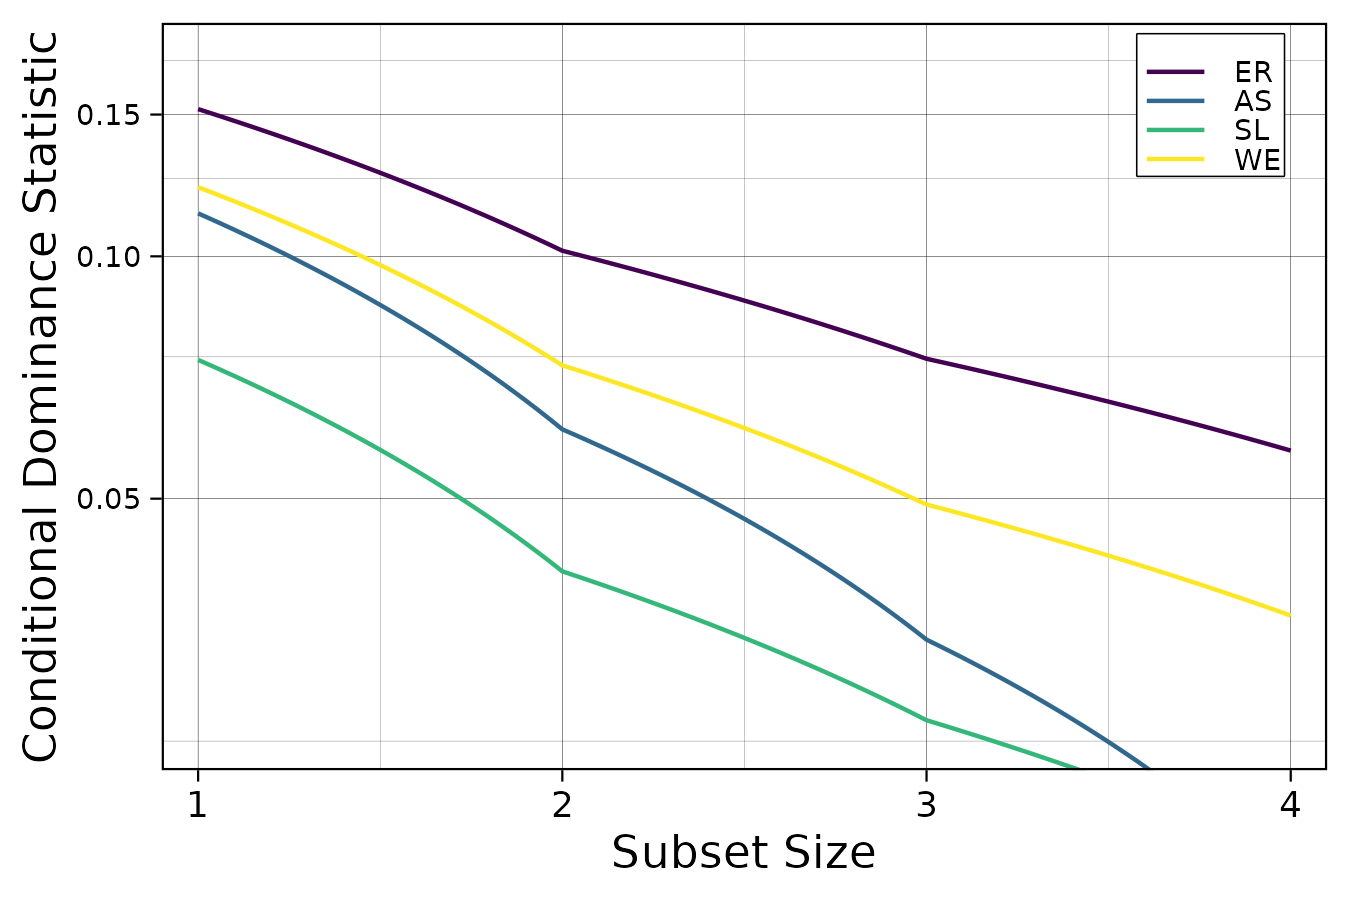
\includegraphics{includes/condit_gph}
		\label{fg:cdl}
	\end{figure}

	The graphic format is useful for the reporting of conditional dominance statistics with only a few IVs as the relative orientation of each of the lines reflects the nature of the conditional dominance designation implemented in Equation \ref{eq:cdldom}.
	Specifically, if an IVs conditional dominance trendline is always above, and thus never crosses over, another IV's conditional dominance trendline, the IV that is above conditionally dominates the one below.
	Figure \ref{fg:cdl} confirms the complete dominance results in that equipment reliability's line is above the lines for the other three IVs indicating that it dominates each of them.
	Similarly, work experience's line is above skill level's line consistent with the complete dominance results.
	In addition, work experience's line is above assistant staffing's line indicating that it conditionally dominates assistant staffing.
	Although work experience does not explain more than assistant staffing in all comparable models (see Table \ref{tab:r2sub}; specifically, $SJ \sim AS + SL$ versus $SJ \sim SL + WE$'s values), when considering the average increment by number of IVs included, work experience produces bigger increments to the $R^2_{DEV}$ than does assistant staffing levels. 
	As such, work experience's dominance of assistant staffing is model dependent, but not dependent on IV inclusion order.
	
	The conditional dominance relationships for the last two IVs does not offer a different designation than did the complete dominance results.
	Assistant staffing fails to conditionally dominate skill level given skill level's conditional dominance statistic at subset size 4.
	These conditional dominance results further reinforce the idea that attempting to rank these IVs is not straightforward and their contributions to prediction depend on the order of their inclusion in the model. 
	
	Given that no complete or conditional dominance designations were possible for comparing assistant staffing with skill level, I proceed to evaluating the general dominance designations between these variables. 
	The general dominance statistics for each tailoring shop IV was computed using Equation \ref{eq:genst} and are reported in Table \ref{tab:gen}.
	
	\begin{table}[h!]
		\centering
		\caption{\centering General Dominance Statistics}
		\begin{tabular}{l|r}
			\toprule
			$ER$ & $0.0965$ \\ 
			$AS$ & $0.0560$ \\ 
			$SL$ & $0.0399$ \\ 
			$WE$ & $0.0700$ \\ 
			\bottomrule
		\end{tabular}
		\label{tab:gen}
	\end{table}

	Evaluating the general dominance designations implied by the general dominance statistics in Table \ref{tab:gen} using Equation \ref{eq:gendom} again shows that equipment reliability dominates each other variable and that work experience dominates skill level and assistant staffing. 
	The general dominance statistics add to the prior dominance designations by determining that assitant staffing generally dominates skill level.
	The general dominance designations then add to the results above in that they allow for a clear rank ordering of the tailoring shop IVs in predicting sport jackets with equipment reliability being the most important followed by work experience, then assistant staffing, and ending with skill level.
	
	In conclusion, the DA results have built on reports of the model in Table \ref{tab:poisreg} by adding additional information about how each of the tailoring shop IVs explains variation or information in the sport jacket production variable. 
	The DA results work to support the inference about the large IRR value obtained by equipment reliability, confirming that this variable, regardless of the order in which it might be included in the model, is most important. 
	In addition, equipment reliability is associated with nearly one-third (i.e., $\frac{.0965}{.2624} \approx \frac{1}{3}$ of the explained information in sport jackets alone.
	The DA results also provide useful contextualization of the other three IV's IRR values from Table \ref{tab:poisreg}.
	Specifically, the IRR values for work experience, assistant staffing levels, and skill level were similar, each within .01 of one another. 
	It would then seem like each IV might have a similar importance comparison with each other IV.
	The dominance designations obtained showed this is not the case as work experience completely dominated only skill level and conditionally dominated assistant staffing levels. 
	Moreover, assistant staffing levels generally dominated skill level.
	The DA results then showed a great deal of variability in terms of strength of dominance designations even within this rather narrow window of IRR values.

	\subsubsection{Section Summary}
	
	This section provided an extensive analytic walk through of a data analysis in a PR model using simulated data.
	The PR model described in this section interpreted model coefficients using IRRs and applied the recommended DA methodology using the $R^2_{DEV}$ to dominance statistics and designations.
	
	The data analytic conditions under which the PR model above was generated and estimated assumed that the time window under which each tailoring shop was observed was two weeks.
	In many real world situations involving count DVs, the time window might vary from observation to observation. 
	Under such conditions, the observations are "exposed" to the count generating mechanism differently.
	In the section below, I shift the focus to a conceptual discussion of what exposure means for count DVs, how differential exposure is accommodated in CRMs, and offer an example of differential exposure affects DA statistics and designations with another data analytic example.
	
\section{Additional Consideration for CRMs}

	CRMs are defined by their accommodation of the semi-continuous and non-negative values on which count DVs take.
	Count DVs, in addition to these two facets, are also marked by an implied level of aggregation.
	Note that all the count DVs discussed in the introduction, as well as the simulated DV in the example above, all aggregate a number of events over a specific period of time.	
	
	That count DVs as aggregated events is a common interpretation of a Poisson distributed variable. 
	Indeed, Poisson variables can be defined as accumulated repeated sampling from a Binomial distribution with a set probabity of occurrence and a set number of trials \cite(e.g.,){hodges1960poisson}.
	In this interpretation of the Poisson, the Poisson mean parameter $\mu$ is the product of the number of trials $n$ for the Binomial distribution times the probability $p$ of the event occurring in the Binomial distribution.
	Given the Binomial interpretation of the Poisson, it is clear that CRMs assume that the counts of events realized in the data are derived from Binomial processes that share the same number of trials and probabilities of occurrence.
	The linkage between aggregated Binomial processes and the negative Binomial distribution is even clearer as it is, in fact, defined as aggregated Binomial events or trials.
	In the end, both PR and NBR models can be seen as a method for modeling aggregated event counts that stem from a specfic set of Binomial processes.
	
	That count DVs can differ in their exposure to, or the number of trials in producing, the observed count values is can be accommodated in the analysis assuming that the differences in exposure to the count generating processes are encoded into a variable that can be used to adjust the results of the CRM.
	In the section below, I elaborate more on what differential exposure is, the practical effects of differential exposure on answering research questions with count DVs, and how to adjust CRM results to ensure that count DVs that might be affected by differential exposure produce accurate DA statistics and designations.

	\subsection{Differential Exposure and Offset Terms}
	
	Analysis of data with CRMs is, fundamentally, a method to answer research questions.
	Consider, for example, evaluating whether a customer service training increases the number of positive reviews for a business.
	From the perspective of the Binomial interpretation of count events like positive reviews, the researcher must consider whether the training will affect the probability of receiving a positive review from any given customer, the number of customers who can provide a review, or both factors.
	For this research question, the customer service training is likely to be most relevant to the probability of receiving a positive review from any given customer.
	Thus, with a fixed set of customers, the customer service training should increase the count of positive reviews due to increasing the probability that any one customer is happy and thus provides a positive review.
	
	A complication that can easily arise in evaluating a research question like the one above is that two business locations can have different numbers of customers.
	If location A has 100 customers and location B has 1,000 customers, I would expect that location B would have more positive reviews that location A given the same underlying probability of observing the postitive review event.	
	The count DV, however, does not naturally contain this information and, in fact, the default CRM assumption is that that the two locations have the same number of customers---a fact known not to be true.
	
	That both locations have different numbers of customers means that the locations have different levels of exposure or 'differential exposure' to the count generating probability. 
	The differential exposure in locations A and B is a problem when interpreting the count DV for answering the research question. 
	Consider what would happen in a CRM if locations A and B both receive 10 positive reviews.
	I know that both values of 10 imply starkly different probabilities of observing an event (i.e., $\frac{10}{1000} = .01$ and $\frac{10}{100} = .1$).
	The CRM, however, does not have any built-in way to distinguish between the location's values given just the count DV values and they would be erroneously treated the same in the model.
	What the CRM needs is to be instructed how to adjust the results for the known differential exposure that obscures the differences in the underlying probability of event occurrence.
	
	CRMs can control for differential exposure using an offset term.  
	The offset term, for a log-linear CRM, is natural log transformed version of a variable that reflects the known differential exposure between observations set to a coefficient value of 1.
	Thus, to control for differential exposure, the researcher must have access to a variable that reflects, for each observation, the exposure that the observation had to the count generating process.
	When this exposure variable is natural logarithm transformed and included in the CRM with a coefficient of 1, the DV predicted by the model becomes the ratio of counts out of the value of the exposure or the rate of events given exposure.
	
	The transformation of the count DV to a rate follows is easier to see when making a few algebraic manipulations to the model.
	Consider the most simple case of a CRM, an intercept only model that is fit with an offset term.
	An intercept-only model with an offset would, as a formula, look like: $Y = e^{\beta_o\ln X_{exposure} + \beta_1}$, where $X_{exposure}$ is the exposure variable, $\beta_1$ is the offset term, and $\beta_1$ is the model intercept.
	Taking the natural logarithm of both sides of the equation and given the offset term is 1, the equation above simplifies to $\ln Y = \ln X_{exposure} + \beta_1$.
	Subtracting $\ln X_{exposure}$ from both sides results in $\ln Y - \ln X_{exposure} = \beta_1$.
	Finally, the difference between two logarithms is the logarithm of their quotient, thus producing $\ln \frac{Y}{X_{exposure}} = \beta_1$ or $\frac{Y}{X_{exposure}} = e^{\beta_1}$.
	The natural logarithm transformed exposure variable, when included with an offset term, necessaily results in the dependent variable being a rate.
	
	The practical effect of the offset term is that the DV better reflects the underlying probability of the event and is no longer contaiminated with different levels of exposure to the count generating process.
	An additional side effect of the offset term is that it reduces the extent of unexplainable variation, or deviance, in the count DV.
	The reduction in unexplainable variation arises as observations with high counts and high exposure values are pulled nearer those with low counts and low exposure values.	
	As a result of the reduced unexplainable variation, inclusion of an offset term affects the values obtained $R^2_{DEV}$ values and DA statistics on which they are based.
	
	In the sections below, I show the effect differential exposure has on the results of CRMs when by repeating the analysis applied to the sport jacket production variable to two new Poisson distributed variables.
	These two new variables are based on the same underlying causal model as sport jacket production variable above but have been contaminated with two different kinds of differential exposure.
	My intention in providing examples of the effect of multiple kinds differential exposure on count DVs is to illustrate the likely result of such differential exposure on model coefficients as well as DA designations and statistics.
	I also show how the inclusion of an appropriate offset term can correct such differential exposure contamination across all forms of results.
	
	\subsection{Dominance Analysis with Offset Terms: Analytic Examples}
	
	This section extends on the data analysis of the sport jacket production variable by developing two additional sport jacket production variables that were observed under time periods with different types of holidays.	
	As above, the generation perspective and actual implementation of generating these variables is described in the online supplement as opposed to in this manuscript directly. The section below describes the two new variables, and their contaminating differential exposure processes, prior to using them in analysis.
	
		\subsubsection{Data Generation}
		
	The focus in this section remains on evaluating the effect of the four tailoring shop characteristics in predicting stock jacket production from the same set of 6,780 tailoring shops as above. 
	The difference in the count variables produced below are that they were measured during different two-week periods with different kinds of holidays.
	
	One of the two-week periods in which these tailoring shops were observed occurred near a religious holiday that is not celebrated in the same way by all tailoring shops.
	The resulting sport jacket production variable under religious holiday observance (called $SJ_{RH}$ below) was contaminated by differential exposure owing to inconsistent leaves of absence by tailors over the two-week period.
	These inconsistent leaves of absence made for each tailoring shop having different numbers of days in which no work was done and, thus, no exposure to the probability generating process.
	Assume in this case that it is known that the observance of the religious holidays in this period of time are uncorrelated with any of the tailoring shop characteristics. 
	Thus, the differential exposure process contaminating the sport jacket production variable with religious holiday observance is completely random.
	
	The second of the two-week periods in which these tailoring shops were observed occurred near a time when it is common for tailoring shops to take voluntary holidays
	The resulting sport jacket production variable under voluntary holiday (called $SJ_{VH}$ below) was also contaminated by differential exposure owing to inconsistent leaves of absence by tailors over the two-week period.
	Assume in this case that it is known that taking voluntary holidays depends on tailoring shop characteristics.
	Tailoring shops with specific characteristics were more likely to take holidays during this two-week period than other shops.
	Thus, the differential exposure process contaminating the sport jacket production variable taking a voluntary holiday is completely correlated with the tailoring shop characteristics.
	
	The means, standard deviations, and correlations of the new sport jacket production variables with each of the tailoting shop IVs are reported in Table \ref{tab:dscEx}.
	
	\begin{table}[h!]
		\centering
		\caption{\centering Descriptive Statistics with Differential Exposure}
		\begin{tabular}{lrrrrrr}
			\toprule
			&  &  Standard & \multicolumn{4}{c}{Correlations} \\ 
			\cmidrule(lr){4-7}
			Variable & Mean & Deviation & $ER$ & $AS$ & $SL$ & $WE$ \\ 
			\midrule
			$SJ_{RH}$ & $0.5448$ & $0.7610$ & $0.3290$ & $0.2875$ & $0.2291$ & $0.2977$ \\  
			$SJ_{VH}$ & $0.4876$ & $0.6754$ & $0.2265$ & $0.2084$ & $0.1328$ & $0.2254$ \\
			\bottomrule
		\end{tabular}
		\label{tab:dscEx}
	\end{table}
	
	The two types of holidays described above have the effect of making fewer working days and thus will reduce the magnitude of the mean and standard deviations of Poisson distributed variables like the sport jacket production variables.	
	Consistent with that expectation, by comparison to the results in Table \ref{tab:desc}, Table \ref{tab:dscEx}'s results, show that the means and standard deviations for sport jacket production shrunk given the two types of holidays.
	
	The two types of holidays would also be expected to have specific effects on the correlations with the tailoring shop characteristics.
	The random religious holiday observance differential exposure is likely to shrink correlations with all tailoring shop characteristics.
	This is because this random differential exposure effectively adds unexplainable error variation to the sport jacket production process.
	By contrast, the tailoring shop characteristic-correlated voluntary holiday differential exposure should change the magnitude of the correlations consistent with the exposure process.
	When comparing the correlations in Table \ref{tab:desc} to those of Table \ref{tab:dscEx}, both expected patterns emerge.
	Religious holiday observence shrinks the magnitude of the correlations but does not change the relative magnitudes meaningfully.
	Voluntary holidays however do change the relative magnitudes.
	
	The next section uses the religious holiday observence/random differential exposure-contaminated sport jacket production variable as the dependent variable in a PR as well as a PR-based DA.
	Two different versions of this model are reported.
	One version of the model uses the known religious holiday exposure variable in an offset term and the other does not.
	Both models are reported and compared to show the effect of the inclusion of the offset term for model results.
	
		\subsubsection{Random Differential Exposure}
		
	The two models using religious holiday contaminated sport jacket production are reported in Table \ref{tab:unexp}.
	Only the coefficients, IRRs, and general dominance statistics are reported for each IV for brevity.
		
	\begin{table}[h!]
		\centering
		\caption{\centering Poisson Modeling Results under Random Differential Exposure}
		\begin{tabular}{l|rrrrrr}
			\toprule
			\multicolumn{1}{l}{} & \multicolumn{3}{c}{Without Offset} & \multicolumn{3}{c}{With Offset} \\ 
			\cmidrule(lr){2-4} \cmidrule(lr){5-7}
			\multicolumn{1}{l}{} & $\beta$ & $e^{\beta}$ & $C$ & $\beta$ & $e^{\beta}$ & $C$ \\ 
			\midrule
			$ER$ & $0.2606$ & $1.2977$ & $0.0672$ & $0.2683$ & $1.3077$ & $0.0824$ \\ 
			$AS$ & $0.1225$ & $1.1303$ & $0.0410$ & $0.1210$ & $1.1287$ & $0.0490$ \\ 
			$SL$ & $0.1066$ & $1.1125$ & $0.0277$ & $0.1125$ & $1.1191$ & $0.0352$ \\  
			$WE$ & $0.1287$ & $1.1374$ & $0.0509$ & $0.1360$ & $1.1457$ & $0.0650$ \\ 
			$Intercept$ & $-0.7812$ & $0.4579$ & & $-2.4914$ & $0.0828$ & \\ 
			\bottomrule
		\end{tabular}
	\label{tab:unexp}
	\end{table}
	
	Table \ref{tab:unexp}'s results show that the effect of random differential exposure with religious holiday observance did not substantially affect the IV coefficient and IRR estimates and the results with and without offsets are similar to one another and to the results in Table \ref{tab:poisreg} where there is not differential exposure.
	The coefficients that do change in a noteworthy way are the $Intercept$ values across models with the model omitting the offset obtaining a value near the mean of the religious holiday observance stock jacket production distribution and the model with the offset nearer the underlying probability of observing a stock jacket being produced in any given day in the two-week period (the underlying probability is .1; see online supplement for a discussion).
	
	In addition, the relative comparisons between the IVs' general dominance statistics did not change meaningfully given the random differential exposure with or without the offset term. 
	The most noteworthy result is that all of the DA statistics obtained under random differential exposure in Table \ref{tab:unexp} are smaller compared to those in Table \ref{tab:gen} obtained under equal exposure.
	Thus, irrespective of the use of an offset term, differential exposure affected the magnitude of the general dominance statistics, shrinking them all toward 0 relative to the data obtained under equal exposure.
	
	Although the results obtained with and without an offset term showed a similar pattern of results, the results with an offset term tended to be closer in their values to the data obtained under equal exposure.
	As was noted above, differential exposure adds variation to the model deviance that is unexplained in the absence of an offset term.
	The difference in the magnitude of the general dominance statistic values obtained with and without an offset term reflect this effect.
	When the offset term is not included there is more variation in the model that is unexplained, reducing the magnitude of the $R^2_{DEV}$.
	By contrast, when the offset term is included, the additional variation introduced by differential exposure is reduced which has the effect of increasing the $R^2_{DEV}$.
	
	The section below transitions away from random differential exposure to the correlated differential exposure mechanism introduced by taking voluntary holidays.
	Again, correlated differential exposure is the process where the exposure variable is related to the IVs in the statistical model.
	Given these relationships, the effect of correlated differential exposure on the model results is expected to be more substantial.
	As with the random differential exposure results, the correlated exposure results include a model with an offset and without an offset.
	
		\subsubsection{Correlated Differential Exposure}
		
	The two models using voluntary holiday contaminated sport jacket production are reported in Table \ref{tab:exp}.
	As before, model coefficients, IRRs, and general dominance statistics are reported.
	
	\begin{table}[h!]
		\centering
		\caption{\centering Poisson Modeling Results under Correlated Differential Exposure}
		\begin{tabular}{l|rrrrrr}
			\toprule
			\multicolumn{1}{l}{} & \multicolumn{3}{c}{Without Offset} & \multicolumn{3}{c}{With Offset} \\ 
			\cmidrule(lr){2-4} \cmidrule(lr){5-7}
			\multicolumn{1}{l}{} & $\beta$ & $e^{\beta}$ & $C$ & $\beta$ & $e^{\beta}$ & $C$ \\ 
			\midrule
			$ER$ & $0.1706$ & $1.1860$ & $0.0305$ & $0.3081$ & $1.3608$ & $0.0881$ \\ 
			$AS$ & $0.0934$ & $1.0979$ & $0.0217$ & $0.1381$ & $1.1480$ & $0.0512$ \\
			$SL$ & $0.0402$ & $1.0410$ & $0.0076$ & $0.1166$ & $1.1236$ & $0.0323$ \\ 
			$WE$ & $0.1096$ & $1.1158$ & $0.0311$ & $0.1527$ & $1.1650$ & $0.0677$ \\
			$Intercept$ & $-0.8011$ & $0.4488$ & & $-2.4769$ & $0.0840$ & \\
			\bottomrule
		\end{tabular}
		\label{tab:exp}
	\end{table}
	
	As compared to the random differential exposure results in Table \ref{tab:unexp}, the correlated differential exposure results in Table \ref{tab:exp} show clear differences in patterns of results across models with and without an offset term.
	The correlated differential exposure effect in the model without an offset has changed the coefficients' absolute values noticeably, shrinking all IRR values but most substantially for equipment reliability.
	By contrast, the model with the offset term obtains coefficient values that are, generally, more similar relative to one another as the data under equal exposure especially for the equipment reliability and skill level IVs.
	This change in the relative magnitude of the coefficients in the model without an offset is the result of the IVs now having two ways in which to predict the sport jacket production outcome: the traditional path where the IV increases the probability of obtaining a sport jacket in a given day and, in addition, the exposure path where the IV increases the probability of any given day being a non-work day; thus, not having the chance to produce any sport jackets.
	When the offset term is included, the second, exposure path is controlled for in the model, and the model again reflects only the effect of each IV on the probability of producing a sport jacket on any given day.
	
	A crucial change in the results for the data under correlated differential exposure is that the dominance designations shift in the model without an offset term relative to the model with an offset term.
	Without an offset, work experience is the most important variable overall, swapping places with equipment reliability. 
	By contrast, the results with an offset term mirror those from the data under equal exposure with equipment reliability being designated the most dominant IV.
	It is also important to note that the dominance statistics across random and correlated differential exposure models with an offset term are very similar to one another and to the results from the data under equal exposure.
	Taken together, these results help to illustrate the value of including the offset term for the accurate computation of DA designations and statistics.	
	
		\subsubsection{Section Summary}
		
	This section discussed the impact of differential exposure on the results of CRMs with a focus on DA designations and statistics.
	I have argued that when a researcher is interested in using a count DV to answer a research question that focuses on increasing the probability of observing the event that produces counts, that differential exposure to the probability can lead to contamination of the count DV and should be corrected using an offset term.
	
	The impact of differential exposure to the probability generating process was illustrated using two different count DVs with different differential exposure mechanisms.
	One mechanism was a random differential exposure mechanism.
	This random differential exposure was reflected by religious holiday observance on sport jacket production among the tailoring shops.
	The random differential exposure affected the model results primarily by adding in additional unexplainable variation to the count DV that is reflected in the magnitude of the DA statistics.
	
	The other mechanism was a correlated differential exposure mechanism that was dependent on the levels of the tailoring shop characteristics.
	This correlated differential exposure was reflected by taking voluntary holiday leave on sport jacket production among the tailoring shops.
	The correlated differential exposure affected the model results more directly by producing an alternative mechanism for sport jacket production which affected model coefficients as well as DA designations and statistics.
	
	A key takeaway from this section is that the use of offset terms is an effective way to recover more accurate DA designations and statistics when the focus of the research is on the probability of events and the count DV is contaminated with differential exposure.

	
\section{Discussion}

	In this manuscript I have recommended a methodology for determining the relative importance of IVs in CRMs.
	Specifically, I recommend the DA methodology as an approach that is comprehensive in the information it provides about IV's prediction and, when using an appropriate fit metric such as the $R^2_{DEV}$, can apply to CRMs and provide information analogous to the explained variance $R^2$ using the LRM.
	
	In addition, I walk the reader through an example data analysis applying PR to simulated data. 
	In walking the reader through this example, I use the recommended DA with $R^2_{DEV}$ fit statistic approach to evaluate the relative importance of the four IVs in the simulated data.
	This walk through of the DA focuses on interpreting IV importance with a focus on how meeting different levels of DA designation stringency offers different evidence for the importance of the IVs over one another.
	
	Finally, I discuss differential exposure to count generating processes in CRMs as a potentially biasing factor both for DA statistics and designations.
	In the example analyses discussed that focus on differential exposure, I show that the use of an offset term is effective for recovering more accurate DA statistics and designations and should be used to correct for differential exposure in CRMs when it is likely to affect a count DV.
	
	In combination, this manuscript picks up where Blevins et al. \citeyear{blevins2015count} had left off by recommending the use of a specific postestimation method, DA, for better understanding model prediction as well as expanding on specific issues that affect CRMs
	It remains important to continue to consult their work when choosing to implement a CRM to choose the most appropriate one given the nature of the data.
	I recommend that you follow the estimation of the CRM with a DA to more fully understand and contextualize the predictions made by each IV.
	
	I have touched on many of the key aspects necessary for extending DA to CRM in this manuscript but acknowledge that I have not been able to discuss all relevant issues for determining IV importance in CRMs.
	Below I discuss some noteworthy limitations and additional extensions of this work before closing.
	
	\subsection{Limitations and Future Directions}
	
	In this work, I use only a series of PR models with simulated data to provide empirical examples.
	The use of PR with simulated data was an intentional choice to avoid the need to work through many of the decision points outlined by Blevins et al. \citeyear{blevins2015count} related to the selection of the appropriate CRM.
	In addition, the use of simulated data allowed for designing an underlying dataset that had specific properties---which was especially helpful for the section discussing differential exposure.
	It is important to note again that the same modeling processes applied to an NBR is discussed in the online supplement.
	The results of the NBR-based DA are very similar to those of the PR-based DA given the same underlying data generating model.
	As such, I did not see adding it to the main manuscript as worth the space it would take to describe and have left it in the supplement for any interested reader.
	I will acknowledge before moving on that the use of the simulated data as I have done in this manuscript adds additional complexity to following along with the methodology in the online supplement.
	That said, all the procedures used to simulate the various count DVs are fully replicable, well-documented, and available as a markdown that can be used by interested readers with a working knowledge of R \cite{R}.
	
	A key contribution of this manuscript is in discussing the effect of differential exposure on DA statistics and designations.
	As was shown, differential exposure can bias DA results irrespective of whether the IVs are correlated with the differential exposure process or not.
	I did not provide an extensive evaluation of the effects of differential exposure on CRM coefficients or DA statistics but rather provide a high-level conceptual discussion of the issue and illustration of what can occur in situations where an offset term correction is not applied.
	Although a thorough evaluation of the potential bias introduced by omitting an offset term when differential exposure has contaminated the count DV was not undertaken in this work, I see future research focusing on this issue as applied to DA of potential value and help researchers identify situations when such bias is more or less likely to occur.
	One suggestion for such research would be to implement it in a way similar to Braun, Converse, and Oswald's \citeyear{braun2019accuracy} evaluation of measurement reliability and sampling error on dominance statistics in meta-analytic LRM.
	
	Prior work on DA has also suggested the application of bootstrapping to estimate standard errors for general dominance statistics and reproduce-ability values for other dominance designations \cite{azen2009using,braun2019accuracy}. 
	Bootstrapping the CRM-based dominance statistics and designations is possible for CRM-based DA in the same way as was outlined for logistic regression by Azen and Traxel \citeyear{azen2009using} but is not examined in the present work.
	A substantial complication with the application of standard errors to DA statistics is in providing clear, compelling rationale as to the differences in roles that null hypothesis testing plays in testing coefficients as compared to DA statistics.
	At current, the literature does not offer useful guidelines about how the roles of each type of hypothesis test might affect the interpretation of the model and the research questions it seeks to answer.
	
	Finally, zero-inflation is a commonly observed condition in count DVs that has been discussed extensively in prior work \cite(e.g.,){blevins2015count}. 
	Cameron and Windmeijer \citeyear{cameron1996r} discuss the application of the $R^2_{DEV}$ to zero-inflated CRMs and, thus, a DA methodology based on the same general approach as discussed above could be applied to zero-inflated CRMs.
	One additional complication that arises with considering how to determine importance with zero-inflated models is that zero-inflated CRMs model two processes in the data. 
	The first process is the standard count generating process whereby IVs increase or decrease counts of the DV.
	The second is an "opt out" process whereby IV increase or decrease the likelihood of the count being 0.
	An additional complication introduced by the two processes modeled by zero-inflated CRMs is that it is possible to allow specific IVs to predict the count generating process, the opting out process, or both.
	In such circumstances the researcher should consider whether an alternative approach that emphasizes parameter estimates as opposed to IVs is better suited to the importance determination with DA \cite{luchman2020relative}.
	
	\subsection{Conclusion}
	
	DA is a useful post-estimation methodology for determining the importance of IVs in statistical models such as CRMs.
	This manuscript has provided a recommended methodology for extending DA to CRMs, offered extensive examples focusing on the interpretation of DA statistics and designations with simulated data, and provided recommendations for how to adjust a CRM-based DA when observations in the count DV may have different levels of exposure to the count generating process.
	In combination, the conceptual discussion of DA, CRMs, and differential exposure, when combined with the empirical examples, will provide organizational and other behavioral scientists the necessary tools for better understanding the CRMs they estimate as applied to the research questions to which the results apply.

\bibliography{CountDominance.bib}
\bibliographystyle{mslapa}
	
\end{document}